\section{Discussion\label{sec-lch-eps-discussion}}
\subsection{Growth on \XYL{}\label{subsec-lch-eps-disc-xyl-hts}}
The amount of 135 well-growing strains of all the 191 strains tested corresponds to \py{"\SIpct{" + str((int(round(100*135.0/191.0,0)))) + "}"}. In a similar screening with the aim of finding polyhydroxybutanoate producers from environmental isolates using \xyl{} as the sole carbon source conducted by \textcite{Lopes2009}, only \SIpct{24} of the strains tested grew on \xyl{}. While \textcite{Lopes2009} took into consideration all the strains, in the screening discussed here, only pre-selected strains were used. For these strains the ability to produce \eps{}s was an established fact and most of these strains belonged to genera known for plant pathogenicity. So, the ability to grow in \xyl{} is not uncommon for the strains tested in this screening.

\subsection{High-Content Screening with \XYL{}\label{subsec-lch-eps-disc-xyl-hcs}}
\begin{table}
	\centering
	\setlength{\tabcolsep}{5pt}
	\sisetup{
		table-number-alignment = center,
		table-text-alignment = center,
		table-figures-integer = 1,
		table-figures-decimal = 2,
		table-format = 1.2
	}
	\caption[\XYL{} Consumption by Genus]{\XYL{} consumption by genus. The strains of the plate Xyl1 were incubated in SM17 P30S for \SIh{48} at \SIrpm{1000} and \SIdC{30.0}. The initial \xyl{} concentration was \SIgpl{10.0}. \XYL{} consumption varies among the strains in the range from \enquote{no consumption} to \enquote{complete consumption}. In this table, the consumption is summarized by genus to show that the bacterial genus appears to have a high impact on the \xyl{} consumption. The parenthesized number after the genus name indicates the number of strains belonging to the respective genus on plate Xyl1.\label{tbl-lch-eps-disc-xyl-hcs-c-b-g}}
	% Sum of strains is 94, because E12 = empty and E10 = not grown --> 96 - 2 = 94.
	\begin{tabular}{lSSS[table-format = 2.2]}
		\toprule
		 & \multicolumn{3}{c}{\XYL{} concentration in \si{\gpl}} \\
		\multirow{-2}*{Strain (frequency)} & {Lower quartile} & {Median} & {Upper quartile} \\
		\hline
		\TablesafeInputIfFileExists{data/lch-eps/xyl-hcs/xgt.tex}{}{\fxfatal{File not found: data/lch-eps/xyl-hcs/xgt.tex}}
		\bottomrule
	\end{tabular}
\end{table}

% xyl-hcs: nur Xyl1, da Xyl2 keine vollständige Platte.
\subsubsection{Exclusion of Xyl2}
In the high-content screening with \xyl{}, the plate Xyl1 was tested, while Xyl2 was not. As seen in \vref{tbl-xyl-growth-layout-j}, more than half of Xyl2 was empty, because---as outlined in \vref{sec-xyl-growth}---not all of the strains of the plates EPS1 and EPS2 showed good enough growth on \xyl{}. The complete method for the aldose monomer analysis is quite time-consuming and geared towards the analysis of complete 96-well plates \cite{Ruehmann2015a}. Therefore, Xyl2 was left out from this step of the screening.

The direct screening of the plates EPS1 and EPS2 was not an option either. The high-throughput purification involves a 96-well size exclusion chromatography (see \vref{hteps-purification}) to reduce the overall amount of small molecules (and not just monomeric aldoses) to enable exact quantification and to protect both the HPLC and the MS. Using strains which do not grow on \xyl{} would have meant an additional \SIgpl{10} \xyl{} in the medium. Therefore, the \xyl{} growth screening was used to sort out non-growing strains.

%xyl-hcs: E10 auch am Ende nicht gewachsen? kaum EPS produziert, keine Xylose verbraucht
\subsubsection{Non-Growing Strains}
The strain \xyli{E10} showed growth on an LB agar plate, although it did not grow in the screening. In the \xyl{} growth screening, this strain (\epsi{F7}) grew to a $D_{600}$ of \num{0.63}, three-fold the limit of \num{0.2} and easily visible to the bare eye. One possible explanation is that during the preparation of plate Xyl1, not \epsi{F7}, but \epsj{F7} was transferred. \epsj{F7} was clearly not growing on \xyl{}, with a $D_{600}$ of \num{0.00}. Since only a single strain was affected in this screening, this matter was not investigated in detail. Since \epsi{F7} is designated as \mo{Paenibacillus} and \epsj{F7} as \mo{Gluconacetobacter}, a 16S rDNA analysis would be a suitable method.

%xyl-hcs: E12-Wachstum: bis 2012-11-29 kann davon ausgegangen werden, dass das Ethanol unter der Sterilwerkbank heftigst kontaminiert war mit Sporen; Auswirkungen auf "keine" abgeschätzt, da freies Well ursprünglich gedacht war, um Orientierung der Platte gegen versehentliches Drehen abzusichern und Backgroundwerte zu haben
\subsubsection{Contamination of the Well Xyl1.E12}
Growth in the \enquote{empty} well Xyl1.E12 most likely occurred due to a contamination. As further investigations revealed, the \SIpct{80} ethanol for the replicator had not been replaced for around a month. After incubating \SIml{1} of the ethanol on an LB agar plate for \SIh{48} at \SIdC{30}, several hundred colonies had formed with at least two distinct colony morphologies. The replicator was flamed, but given such a high concentration of spores, it is not unlikely to have inoculated the empty well. As a consequence for all later experiments, only fresh ethanol was used and put into an autoclaved container and the replicator was also autoclaved regularly.

%xyl-hcs: Xyloseverbrauch: grundsätzliche Anmerkungen zu vermutlich schlechten (sauerstoffarmen) Wachstumbedingungen
\subsubsection{\XYL{} Consumption}
\nomenclature[formula_OTR]{OTR}{oxygen transfer rate}
The median residual \xyl{} concentration was \py{xyl_hcs_xmed} after \SIh{48} of incubation. Four possible reasons for this relatively high value are discussed in the following: low initial cell count, low oxygen transfer rate (OTR), \eps{} production and the strain-specific growth and \xyl{} consumption characteristics. Additionally, the screening used the same medium for all the different bacteria. Some of them might grow faster, consume more \xyl{} or produce more \eps{} in an optimized medium. As the goal of this work was to find a robust strain, no further efforts were devoted to medium optimization at such an early point.

In the work of \textcite{Ruehmann2015b}, the main culture was inoculated from \SIul{10.0} of the pre-culture, while the main culture of this screening was inoculated using the replicator. Therefore, the initial number of bacteria transferred to the main culture could have been too low for complete \xyl{} consumption.

%Duetz2004: Progression des OTR (* = Originalwert = nicht extrapoliert!):
% n.       e = 50 mm    e = 25 mm    e = 12.5 mm  e = 6.25 mm  e = 5 mm
%  200/min 15*            0*           0           0            0
%  300/min 33*           15*           0           0            0
%  400/min -             30*          15           0            0
%  500/min -             45           30          15            9
%  600/min -             60           45          30           24
%  700/min -             75           60          45           39
%  800/min -             90           75          60           54
%  900/min -            105           90          75           69
% 1000/min -            120          105          90           84
% 
% 5 mm extrapoliert als: Spalte links davon abzgl. Anteil an Halbierung durch Schritt von 6.25 mm auf 5 mm ($wert_links - 15 * (1.25/3.125))
% 
% Duetz2000: Verhältnis von OTR bei 500 µl zu 1000 µl: etwas weniger als die Hälfte --> OTR bei etwa 40 mmol/(l*h) mit 1000/min und 5 mm Exzentrizität (solange nicht viskos)
% The switch from exponential to linear, oxygen-limited growth occurred at biomass concentrations of 5, 4, and 2 g/l for culture volumes of 500, 750, and 1,000 µl respectively.
Microbial growth in deep-well plates at \SIrpm{1000} and an eccentricity of only \SImm{5} might have been limited by an insufficient OTR \cite{Duetz2000, Duetz2001, Duetz2004, Hermann2003}. Extrapolating\footnote{
Every time the eccentricity halves, the minimum shaking frequency must be increased by another \SIrpm{100} to reach the same OTR as before. The OTR was treated as increasing linearly from \SIrange{0}{120}{\otrunit} at an eccentricity of \SImm{25} starting from \SIrpm{200} and going to \SIrpm{1000}. The step from \SImm{6.25} to \SImm{5.0} was treated as being the OTR at \SImm{6.25} subtracted by 
$\SIOTR{15} \cdot { \frac{\SImm{6.25} - \SImm{5.0}}{\num{0.5} \cdot \SImm{6.25}} }$.
}
the data presented by \textcite{Duetz2004}, the OTR in a deep-well plate using \SIul{500} filling volume would be \SIOTR{84}. According to \textcite{Duetz2000, Duetz2001}, the OTR ratio of a well with a filling volume of \SIul{500} and \SIul{1000} is between 2:1 and 3:1. This would equate to an OTR in the range of \SIrange{28}{42}{\otrunit}, which is comparable to the OTR achieved in \SIml{250} Erlenmeyer flasks with \SIml{25} medium at \SIrpm{300} and an eccentricity of \SIcm{5.0} \cite{Hermann2003}.

The experimental maximum OTRs of \SIul{200} filling volume given by \textcite{Hermann2003} for 96-well plates shaken at \SIrpm{1000} and an eccentricity of \SImm{3} and \SIrpm{900} and an eccentricity of \SImm{6} were \SIOTR{15} and \SIOTR{24}, respectively. At \SIul{200} filling volume, the OTR without shaking was \SIOTR{7} \cite{Hermann2003}. No values for \SIul{1000} filling volume were reported. Given these numbers, low OTR might have occurred, but taking into consideration that \py{str(len(xyl_hcs_xc[3]))} strains consumed at least \SIpct{85} of the \xyl{}, it seems unlikely to be the sole reason behind low \xyl{} consumption for all strains.

\EPS{} production might increase the dynamic viscosity, which in turn would reduce liquid movement due to shaking and reduce the OTR. Since the 13 strains which produced substantial amounts of \eps{} (see \vref{tbl-xyl-hcs-hits}) consumed \xyl{} to levels of \SImgpl{665} at most, it is highly unlikely that \eps{} production adversely affected \xyl{} consumption. On the contrary, \textit{all} \eps{} producing strains readily consumed \xyl{} leading to the hypothesis that good \xyl{} consumption generally positively affects \eps{} production in certain types of strains.

Therefore, the reason for differences in \eps{} production and \xyl{} consumption has to lie within the bacteria used. The data presented in \vref{tbl-lch-eps-disc-xyl-hcs-c-b-g} support this statement. The table lists the median residual \xyl{} concentrations for each bacterial genus and while some genera such as \mo{Microbacterium}, \mo{Paenibacillus} or \mo{Pseudomonas} were able to consume \xyl{} almost completely, others such as \mo{Sphingomonas} did show low \xyl{} consumption at best.

%xyl-hcs: Unterschiede in der EPS-Produktion auf Xylose
\subsubsection{Differences in \EPS{} Production}
Only thirteen strains produced reliably detectable amounts of \eps{} which were measured as aldose monomers (see \vref{xyl-hcs-subsec-amc}). While the strains of the \eps{} bank are known to produce different amounts of \eps{} \cite{Ruehmann2015b}, the low \eps{} production on \xyl{} was still peculiar. The median cumulative aldose monomer concentration across all strains tested was at \SImgpl{102}, lower and upper quartiles at \SImgpl{68} and \SImgpl{208}, respectively. % Source: data/xyl-hcs/full.py
The same strains grown on \glc{} \cite{Ruehmann2015b}, exhibited similar productivity with median, lower and upper quartiles at \SImgpl{86}, \SImgpl{45} and \SImgpl{318}, respectively, and 20 strains reaching at least \SImgpl{560} cumulative aldose monomer concentration. % Source: data/discussion/Xyl1_BR_EPS_CAMC.txt + Analysis in LO
The maximum concentrations were also not affected. Therefore, it can be concluded that the productivity on a plate scale was mostly unaffected.

%xyl-hcs: UNterschiede in EPS auf Xyl/Glc
\subsubsection{Differences in \EPS{} \AMC{}\label{subsubsec-lch-eps-disc-diff-eps-amc}}
The influence of the carbon source on the aldose monomer composition of the \eps{}s has been examined using \glc{} versus \xyl{}. As seen in \vref{fig-lch-eps-xyl-vs-glc}, only two of the 13 strains showed major differences in the \eps{} \amc{} when grown on \xyl{} compared to \glc{}. Two strains showed minor differences and the remaining strains appeared to be unaffected.

To the best of my knowledge, there are no reports on the screening and comparison of the \eps{} \amc{} of \eps{} producers grown on \glc{} and \xyl{} in the published literature so far. However, several authors have found differences in the \eps{} composition of different microorganisms grown on different carbon sources \cite{Kai2003, Lee1995, Lee2007, Grobben1996, Grobben1997, Cerning1994, Fischer2003, Osman1986, Bryan1986, Raza2011, Tait1986}.

\nomenclature[latabbr_NMR]{NMR}{nuclear magnetic resonance}
\textcite{Kai2003} studied the fungus \mo{Pestalotiopsis microspora} and the composition of its \eps{} grown on \glc{}, \man{}, \gal{}, \xyl{}, \glcnac{}, \rha{}, \lara{} and \dara{} using gas chromatography and \ce{^{13}C}~NMR. The \eps{} contained at most three monomers: \man{}, \glc{} and \gal{}. The resulting \eps{}s can be divided into four groups, based on the carbon source used: group 1 with \glc{}, \man{}, \rha{} and \dara{}; group 2 with \gal{}; group 3 with \xyl{} and \glcnac{} and group 4 with \lara{}.

The group 1 \eps{}s contained \SIpct{90} \glc{} and \SIpct{10} \man{}, while the group 2 \eps{} contained slightly more \man{}, around \SIpct{15}. The \eps{}s of group 3 were the only ones to contain \gal{} at \SIrange{10}{15}{\percent}. \GLC{} was at \SIrange{55}{60}{\percent} and the remaining \SIrange{25}{35}{\percent} were made from \man{}. The group 4 \eps{} contained \glc{} exclusively. All of these results are in \si{\molpercent}.
%\cite{Kai2003}: \mo{Pestalotiopsis microspora}; EPS composition (man vs. glc. vs gal.) vs. C source (glc vs. man vs. gal vs. xyl vs. glcnac vs. rha vs. l-ara vs d-ara). glc vs. man vs. rha vs. d-ara = equal/very similar; gal bit more man than in glc/man/rha/d-ara; xyl vs. glcnac = contain gal, similar; contain considerably more man; l-ara: 100\% glc

The fungus \mo{Phellinus linteus}~L13202 was studied by \textcite{Lee1995} and the growth, \eps{} production and composition on different carbon sources, among them \glc{} and \xyl{}. Unfortunately, the fungus did not grow in \xyl{}, therefore, no \eps{} was produced and hence, no compositional data reported.
%\cite{Lee1995}: \mo{Phellinus linteus} L13202 (fungus); EPS vs. C source (glc vs. gal vs. man vs. ara vs. starch). all similar; glc vs. man = equal; boring

Another fungus, \mo{Ganoderma applanatum} was studied by \textcite{Lee2007}. While they did not test \xyl{} as a carbon source, they found up to \SIpct{10} of \xyl{} in the polymer.
%\cite{Lee2007}: \mo{Ganoderma applanatum} (fungus): glc vs. mal vs. frc vs. saccharose: differences not discussed: \enquote{The sugar compositions of EPS and PPS varied with the carbon sources. It is possible that different carbon sources might have different effects of catabolic repression on the cellular secondary metabolism.} \XYL{} part of the polymer, other three are \glc{}, \man{} and fructose. Values are in mass-\%! No reference papers for EPS composition found.

The lactobacillal \eps{}s of \mo{Lactobacillus delbrueckii} subsp. \mo{bulgaricus}~NCFB~2772 and \mo{Lactobacillus casei}~CG11 were studied by \textcite{Grobben1996, Grobben1997} and \textcite{Cerning1994}, respectively. The carbon sources studied were \glc{} and \frc{} \cite{Grobben1996, Grobben1997}, and \glc{} and lactose \cite{Cerning1994}.

It was found that on \frc{}, the \eps{} of \mo{Lactobacillus delbrueckii} subsp. \mo{bulgaricus}~NCFB~2772 consisted of \glc{} and \gal{} in the ratio 1:2.4, while in an equimolar mix of \glc{} and \frc{} and on \glc{} alone, the composition shifted to \glc{}, \gal{} and \rha{} in the ratio 1:7.0:0.8 \cite{Grobben1996}. After the separation of a high molar mass peak from a low molar mass peak, the high molar mass \eps{} from the same strain grown on \frc{} was composed of \glc{}, \gal{} and \rha{} at a ratio of 1.3:4.3:1.0. On \glc{} the composition shifted to 1:4.7:1 \cite{Grobben1997}.
%\cite{Grobben1996}: Glc vs. frc in \mo{Lactobacillus delbrueckii} subsp. \mo{bulgaricus} NCFB 2772: frc-only (167 mM): glc:gal = 1:2,4; frc-glc mix (each 83 mM): glc:gal:rha = 1:7.0:0.8; glc-only (167 mM): as mix.
%\cite{Grobben1997}: Glc vs. frc in \mo{Lactobacillus delbrueckii} subsp. \mo{bulgaricus} NCFB 2772, two fractions (high molas mass, low molar mass; only high molar mass given here): frc-only (139 mM): glc:gal:rha = 1.3:4.3:1.0; glc-only (139 mM): glc:gal:rha = 1:4.7:1.

Comparing the growth of \mo{Lactobacillus casei}~CG11 on \glc{} and lactose, \textcite{Cerning1994} found that the \eps{} compositions differed: on \glc{}, the polymer consisted of three quarters (\SIpct{75.7}) \glc{}, a fifth (\SIpct{20.5}) \rha{} and traces of \gal{} (\SIpct{2.1}) and \man{} (\SIpct{1.7}). On lactose, the lion's share (\SIpct{63.0}) was still made up of \glc{}, while almost the same amounts of \rha{} (\SIpct{16.1}) and \gal{} (\SIpct{13.2}) were found. The remainder consisted of \man{} (\SIpct{6.8}) and \xyl{} (\SIpct{1.0}).
%\cite{Cerning1994}: \mo{Lactobacillus casei} CG11 (only interesting strain), CG11-NB, CG11-St; EPS vs. carbon source. Lac vs. glc; monomers: rha, fuc, ara, xyl, man, gal, glc. Lac: main sugars Rha, gal, glc; glc most abundant. Glc: main sugars Rha, glc; glc most abundant.

\textcite{Fischer2003} examined the \eps{} of \mo{Azospirillum brasilense}~Cd under \enquote{normal} (minimal medium) conditions and with the addition of wheat root exudate. The \eps{} produced with pure minimal medium contained \SIpct{47} \glc{}, \SIpct{28} \fuc{}, \SIpct{11} \gal{}, \SIpct{6} \rha{} and only traces of \xyl{}, \man{} and \lara{}. However, the \eps{} produced with wheat root exudates looked different: \glc{} was still the major component with \SIpct{37}, but there were considerably less \fuc{} (\SIpct{14}) and \rha{} (trace); on the other hand, \xyl{} (\SIpct{17}) and \lara{} (\SIpct{11}) made up more than a fourth of the polymer. The \gal{} (\SIpct{15}) and \man{} (trace) contents were virtually unchanged.
%\mo{Azospirillum brasilense}~Cd: EPS "normal" \SIpct{47} \glc{}, \SIpct{28} \fuc{}, \SIpct{11} \gal{}, \SIpct{6} \rha{}, traces of \xyl{}, \man{} and \lara{}. Growth on wheat root exudate: \glc{} with \SIpct{37} still major component, but \SIpct{15} \gal{}, only \SIpct{14} \fuc{}, \SIpct{17} \xyl{}, \SIpct{11} \lara{}, traces of \rha and \man{}.

The \eps{} of four strains of \mo{Pseudomonas syringae} pv. \mo{glycinea} grown on saccharose, \glc{} and on soybean leaves were analysed by \textcite{Osman1986}. On saccharose, a levan was produced, while they found an alginate on \glc{} and on leaves.
%\cite{Osman1986}: \mo{Pseudomonas syringae} pv. glycinea, four strains from two "races": semi-synthetic medium (saccharose as carbon source) vs. glc vs. grown on leaves; saccharose: levan formation; glc: high in uronic acid content (50\% to 75\%), mannose (alginate); leaves (only compatible interactions): 32\% to 50\% uronic acid, mannose (alginate).

In 1986, \textcite{Bryan1986} studied \mo{Klebsiella} sp. K32 and \mo{Acinetobacter calcoaceticus}~BD4 on defined media with \glc{}, \man{}, \rha{}, succinate, glutamate or ethanol as the carbon source and a complex medium with \glc{}. In all cases, the relevant monomers of \mo{Klebsiella} \eps{} were \gal{}, \man{} and \rha{}. The molar ratio of \rha{} to \gal{} was 1:2 on ethanol, almost 2:1 on \glc{}, \man{} or \rha{} and approximately 1:1 on the complex medium. \MAN{} was present only when grown on \rha{} and only in trace amounts. The effect on \mo{Acinetobacter calcoaceticus}~BD4 was more pronounced: when grown on \rha{}, the molar ratio of \rha{}:\glc{}:\man{} was approximately 1:1:2 on \rha{}, 4:2:1 on succinate and 10:5:1 on glutamate or ethanol.

%\cite{Bryan1986}: \mo{Klebsiella} sp. strain K32 and \mo{Acinetobacter calcoaceticus}~BD4; EPS vs. growth phase; EPS vs. carbon source. Ratios in table 1 = molar. for each strain: defined medium with glc vs. man vs. rha vs. succinate vs. glutamate vs. ethanol vs. complex medium with glc. for Klebsiella strain: relevant monomers rha vs. gal vs. man. for Acinetobacter strain: relevant monomers rha vs. glc vs. man. Paper macht guten Eindruck. \enquote{The polymer produced by \mo{Klebsiella} sp. strain K32 grown on ethanol had a rhamnose/galactose molar ratio of 1:2. When this strain was grown on defined medium containing glucose, mannose, or rhamnose, however, the rhamnose/galactose ratio was quite different, almost 2:1. When this strain was grown in a complex medium the rhamnose/galactose molar ratio was approximately 1:1.
%
%The sugar composition of the polymer produced by \mo{A. calcoaceticus} BD4 varied dramatically depending on carbon source. The molar ratio of exopolysaccharide produced on rhamnose (rhamnose/glucose/mannose, approximately 1:1:2) was quite different from that produced on succinate (rhamnose/glucose/mannose, 4:2:1) or on glutamate or ethanol (rhamnose/glucose/mannose, 10:5:1).}

\textcite{Raza2011} used the strain \mo{Paenibacillus polymyxa}~SQR-21 to assess the impact of different carbon and nitrogen sources on the \eps{} production. They only analysed the \eps{} composition of the \eps{} produced on an optimized medium. The monomers were \man{}, \gal{}, \glc{} and \glcua{} at a ratio of 2.7:2.5:2.2:1.
%\cite{Raza2011}: \mo{Paenibacillus polymyxa} SQR-21; C/N source vs. EPS production; no C/N source vs. EPS composition (at least, did not report) \enquote{The chemical composition analysis of EPS showed that it contained monosaccharides and glucuronic acid in a ratio of 7.5:1. While amino acids were not detected. For the determination of the monosaccharides composition of EPS, the alditol acetates of polysaccharide were analyzed by gas chromatography. The results revealed that the EPS from SQR-21 was comprised of mannose, galactose and glucose in a ratio of 1.23:1.14:1, respectively (data not shown).}

\textcite{Tait1986} studied the \eps{} production, monomer composition, acetylation and pyruvylation of \mo{Xanthomonas campestris}~S459 with regard to several deficiencies: \glc{}, ammonium, sulphur, phosphorus, magnesium and iron. Under all deficiencies tested, the monomer composition remained constant. The acetyl content of the xanthan remained stable under all conditions tested, except for the ammonium deficiency: the xanthan had the highest acetyl content under this deficiency. Under the same conditions, the lowest pyruvyl content was achieved. The only other deficiency which led to a slight reduction in pyruvyl content was sulphur deficiency.
%\cite{Tait1986}: \mo{Xanthomonas campestris} S459; EPS vs. deficiency (S, ammonium, P, Mg, Glc, Fe). Acetyl content unchanged except high in ammonium-de.f; pyruvyl content down for ammonium-def. (highest acetyl content), slightly for S-def.; monomer composition unchanged

%SUMMARY OF MINI LITERATURE REVIEW
None of the effects observed by \textcite{Kai2003} can be found in the data presented in this work. \textcite{Lee1995} found no growth for the fungus studied on \xyl{}, so that these results cannot be used. \textcite{Lee2007} studied fungi as well and found different \eps{} compositions based on the carbon source, but did not test the carbon sources in question: \glc{} and \xyl{}. The studies of \textcite{Grobben1996, Grobben1997, Cerning1994} with \mo{Lactobacillus} spp. used \glc{}, but not \xyl{}. The same is true for the studies on \mo{Azospirillum brasilense}~Cd by \textcite{Fischer2003}, \mo{Pseudomonas syringae} pv. \mo{glycinea} by \textcite{Osman1986}, \mo{Klebsiella} sp. K32 and \mo{Acinetobacter calcoaceticus}~BD4 by \textcite{Bryan1986}, and \mo{Xanthomonas campestris}~S459 by \textcite{Tait1986}. In the work of \textcite{Raza2011}, the monomer composition was analysed for the optimized medium with \gal{} as the sole carbon source.

However, from the studies which analysed the monomer composition for each carbon source, it can be concluded that the exact culture conditions, more specifically: the carbon source, \textit{can} have a strong influence on the monomer composition. But, the actual extent to which each \eps{} depends on the carbon source and other culture conditions, must be studied in detail for every strain.

It should be kept in mind that \amc{} analyses are just one building block for fostering understanding of microbial \eps{} production capabilities. As \textcite{Ruetering2016} have shown recently, strains harbouring the corresponding genes \cite{Ruetering2017} may produce two different types of \eps{}. Therefore, if one only took into account the \eps{} composition, the conclusion that the composition of \textit{the} \eps{} changed can be misleading.

For none of the strains tested in this screening, additional steps to pinpoint the true nature of apparent differences in the \eps{} \amc{}s were made. Also, no analyses regarding ketoses or modifications with pyruvic or \acet{} were run to keep the workload manageable. From the data available, it cannot be concluded whether different \eps{}s were produced at different levels or if the apparent \amc{}s changed for other reasons. However, the results of the high-throughput screening on \xyl{} presented in this work are in line with the available scientific literature.

\subsection{High-Throughput Screening for Inhibitor Tolerance\label{subsec-lch-eps-disc-inh-tol}}
%inh-tol: Non-growing strains.
\subsubsection{Non-Growing Strains}
Eight strains of the reference did not grow, hence, they had to be excluded from this screening step. The affected strains were neither in the same row nor in the same column, which would have hinted at an operator mistake during pipetting. While the cause is not known and given that in the subsequent very similar experiment with \lch{} all of the affected reference strains grew, a hitherto unknown effect could have caused this: the re-use of deep-well plates.

Some of the deep-well plates used were not new. After use, the previous plate user autoclaved the plate, cleaned it in a lab dishwasher and autoclaved the dry one in a plastic bag again for re-use. Sometimes, additional manual cleaning of single wells was necessary due to stubborn remains from autoclaving. Manual cleaning made extensive use of detergents. Co-workers stated that they also encountered irreproducible growth behaviour in re-used deep-well plates and suspected the cleaning procedure to leave detergents in single wells. The wells in question were filled with cleaning solutions and let to stand overnight. Due to adsorption, even rinsing the plastic afterwards and using the dishwasher might not have removed enough of the detergents. The apparently erratic occurrence of non-growing strains would be in line with the manual cleaning of specific wells only. Unfortunately, no further studies on the phenomenon were performed.

%inh-tol: general problems with statistical power of one measurement for calculating the percentage of inhibitor/reference --> justification; example calculations
%inh-tol: possible interpretation of excessive growth
\subsubsection{Excessively Growing Strains}
Excessive growth was observed for all inhibitors, but \van{}. Generally, excessive growth could be attributed to the utilization of the additional carbon source present. The utilization of \fora{} \cite{Stickland1929, Quayle1972, Friedrich1979}, \acet{} \cite{Herlihy1987, Wright1966}, \fur{} \cite{Brune1983, Boopathy1993, Koopman2010, Lopez2004a, Wierckx2011} and \hmf{} \cite{Boopathy1993, Koopman2010, Lopez2004a, Wierckx2011} are well described. \Laev{} utilization was reported by \textcite{Steinbuechel1997}.

% D600 < 0.8: 39 von 88 in ref1, 29 von 39 in ref2
Growth was measured using the quick, but insensitive method of measuring the attenuance at \SInm{600}. Changes in cell morphology, probably induced by inhibitor presence, could lead to both, over- and underestimation of the growth on the inhibitor. The non-linearity of the attenuance signal was ignored. Assuming that the cell morphology in the inhibitor tests was unaltered compared to the reference, the non-linearity would be cancelled out almost completely at normal growth. Low growth in the presence of an inhibitor would give a better impression than in the linear case, excessive growth in the presence of an inhibitor would give a worse impression than in the linear case.

Since all the growth experiments in inhibitor presence were part of a screening, none of them were reproduced to keep the effort manageable. The probability for false positives and negatives could be high and some of the \enquote{winners} of the inhibitor tolerance screenings could have been selected by chance. For 32 of the 53 excessively growing strains, the reference attenuances were below the average of the plates EPS1 and EPS2 of the growth screening on \xyl{} (\num{0.6}). That at least half of all strains (26.5) grew to the average value is rooted in the definition of the arithmetic mean. The small surplus is explained with random errors. Therefore, excessive growth could also have been caused by a less-than-normal growth of the reference and not only a more-than-normal growth of the strain in inhibitor presence for at most six strains. Nonetheless, the ability to grow in inhibitor presence could still be shown for the strains used in the high-content screening.
%Some wells contained the same strain and only eight strains\footnote{Reference strains with $D_{600} < 0.6$ and growing excessively in more than one inhibitor screening: \xyli{B10}, \xyli{C4}, \xyli{C5}, \xyli{D12}, \xyli{F2}, \xyli{F4}, \xylj{A2}, \xylj{A6}.} made up 19 wells. 
% Utilization of carbon sources: formic acid: Stickland1929, Quayle1972, Friedrich1979; acetic acid: Herlihy1987, Wright1966; furfural: Brune1983, Boopathy1993, Koopman2010, Lopez2004a, Wierckx2011; HMF: Boopathy1993, Koopman2010, Lopez2004a, Wierckx2011; vanillin: none, only degradation, not utilization (Kunc1971, Karmakar2000, Buechert1989, Narbad1998, Gasson1998, Lux1990, Chambers1963); laevulinic acid: Steinbuechel1997.

%inh-tol: how similar are single inhibitor results
\subsubsection{Comparison of Inhibitor Results}
As outlined above (see \vref{intext-lch-eps-overview}), the screening approach was used to quickly reduce the number of strains to test in subsequent screening rounds. For the inhibitor tolerance screening, six different inhibitors were tested. For future re-uses of the strategy employed in this screening, a further reduction of the workload or a higher degree of automation is desirable. Therefore, the results of the different inhibitors are compared in detail in this section to point out potential for refinements.

While only 27 strains showed at least rudimentary growth in the \van{} test series, 17 of these were also present in the top 27/28 of at least one other inhibitor. The exact numbers are: 10 of 27 for \fur{}, 7 of 27 for \hmf{}, 10 of 28 for \fora{}, 10 of 28 for \acet{} and 7 of 28 for \laev{}. Under the assumption that \van{} tolerance is independent from tolerance towards other inhibitors, on average, six\footnote{The amount of strains growing in \van{} presence (27) per all strains tested (127) times the amount of strains in the top 27/28 (27 or 28) rounded to the next integer.
$\frac{27}{127} \cdot 27 \approx 5.74 \approx 6$ or 
$\frac{27}{127} \cdot 28 \approx 5.95 \approx 6$.}
 of the 27 \enquote{\van{} strains} should appear among the best 27 or 28 strains, respectively. This number, six, is smaller than any of the numbers found for the other inhibitors. Although this cannot be considered as solid evidence, it can be used as a hint for reducing the screening effort.

Combining the top strains of \acet{} and \van{} test series, 29 different strains were found. Matches with the top strains of the remaining inhibitors were better than with \van{} alone: 16 of 27 for \fur{}, 14 of 27 for \hmf{}, 13 of 28 for \fora{} and 13 of 28 for \laev{}.

%Acet. + Van.: 29 different strains (Xyl1.A10, Xyl1.B10, Xyl1.C04, Xyl1.C05, Xyl1.C12, Xyl1.D12, Xyl1.E01, Xyl1.E02, Xyl1.F01, Xyl1.F10, Xyl1.G05, Xyl1.G09, Xyl1.G11, Xyl1.H03, Xyl1.H08, Xyl1.H10, Xyl2.A01, Xyl2.A02, Xyl2.A04, Xyl2.A05, Xyl2.A06, Xyl2.A07, Xyl2.A08, Xyl2.A09, Xyl2.B07, Xyl2.B08, Xyl2.C04, Xyl2.C05, Xyl2.C07). Matches Fur.: 16/27 (3); HMF: 14/27 (4); Form.: 13/28 (10); Laev.: 13/28 (14)

Taking the strains of the \hmf{} test series into account as well, the numbers are even better: 22 of 27 for \fur{}, 17 of 28 for \fora{} and 14 of 28 for \laev{}. Three, ten and fourteen strains of the top strains of \fur{}, \fora{} and \laev{}, respectively, were unique across all inhibitors. Subtracting these unique strains, the combination of \acet{}, \van{} and \hmf{} finds all but two, all but one and all strains of the \fur{}, \fora{} and \laev{} test series, respectively. Reducing the amount of inhibitors from six to \acet{}, \van{} and \hmf{} would reduce the workload considerably, while still retaining \SIpct{82}\footnote{All 82 hits of \acet{}, \van{} and \hmf{} and 53 of the 83 hits of the other three inhibitors: $\frac{82 + 53}{82 + 83} = \frac{135}{165} \approx$ \SIpct{82}.} of the hits form the screening.

%Acet. + Van. + HMF: 38 different strains (Xyl1.A07, Xyl1.A10, Xyl1.B10, Xyl1.B11, Xyl1.C02, Xyl1.C04, Xyl1.C05, Xyl1.C12, Xyl1.D02, Xyl1.D12, Xyl1.E01, Xyl1.E02, Xyl1.F01, Xyl1.F04, Xyl1.F08, Xyl1.F09, Xyl1.F10, Xyl1.G05, Xyl1.G09, Xyl1.G11, Xyl1.H03, Xyl1.H08, Xyl1.H10, Xyl2.A01, Xyl2.A02, Xyl2.A04, Xyl2.A05, Xyl2.A06, Xyl2.A07, Xyl2.A08, Xyl2.A09, Xyl2.B07, Xyl2.B08, Xyl2.C04, Xyl2.C05, Xyl2.C07, Xyl2.C12, Xyl2.D02). Matches Fur.: 22/27 (3), Form.: 17/28 (10); Laev.: 14/28 (14)

It should be noted at this point that nine of the fourteen unique strains of the \laev{} test series were among the \laev{} top 14 strains. One interpretation of this is that the metabolic capabilities for \laev{} utilization are usually not tied to \acet{}, \van{} or \hmf{} utilization.

%inh-tol: stickiness of furfural to hydrophobic surfaces, oxidation sensitivity
%\subsubsection{Furfural Adsorption and Oxidation}

%inh-tol: discuss vanillin concentration (hohe Konzentration verhindert Differenzierung zwischen den 100 nicht-wachsenden Stämmen; zudem wenig realistisch hoch
\subsubsection{Inhibitory Effects of \VAN{}}
Most strains were totally inhibited by \van{}: 100 of the 127 strains tested. This also means that the 100 non-growing strains cannot be differentiated further. In hindsight, given that only one strain managed to grow normally, halving the \van{} concentration to \SIgpl{1.0} could have allowed to distinguish between the non-growing strains better and paint a more realistic picture of the metabolic capabilities of more strains.

Prior to the screening, the \van{} concentration of \SIgpl{2.0} seemed to be reasonable to quantify the effect of all phenolic inhibitors encountered in hydrolysates. While \textcite{Jonsson1998} reported the \van{} concentration of a willow hydrolysate to be \SImgpl{430}, \textcite{Clark1984} found the total low molar mass phenolics content in a \mo{Pinus radiata} hydrolysate to be around \SIgpl{2.0}. \textcite{Nishikawa1988} studied the growth and productivity of \mo{Klebsiella pneumoniae} on \xyl{} in the presence of different phenolic inhibitors. For \van{}, they found \SIpct{91.5} growth compared to the reference after \SIh{48}. The inhibitory effects of \van{} on ethanol production in \mo{Saccharomyces cerevisiae} were studied by \textcite{Ando1986} and found to be less severe than those of 4-hydroxybenzoic acid or 4-hydroxybenzaldehyde at \SIgpl{1.0}. They found \SIpct{60} inhibition of \mo{Saccharomyces cerevisiae} at a \van{} concentration of \SIgpl{2.0}.

%inh-tol: Bemerkung über Hydrophobizität von Furfural und PMP-Furfural als Erklärung für Einsatz von Acetonitril im Screeningverfahren
\subsubsection{Acetonitrile Use in HPLC-MS Method}
The methods for \amc{} analysis and aldehyde inhibitor analysis rely on the same basic principle. But, due to the hydrophobicity of the inhibitors, especially \fur{}, and their PMP derivates, it was necessary to use acetonitrile and use a different filter plate to keep the analytes in the solution (data not shown).

\subsection{High-Throughput Screening for \LCH{} Tolerance\label{subsec-lch-eps-disc-lch-tol}}
The single inhibitor screening was conducted as a means to estimate the tolerance towards real world hydrolysate based on single experiments with chemically defined inhibitors. One of the 28 top strains of the \lch{} trial did not grow in the single inhibitor screenings, therefore, only 27 of the 28 strains of \lch{} can be compared with the chemically defined inhibitors. %\fxnote{Comparison of ranks via \cite{Konagurthu2013}?}
Combining all the top 27/28 strains of the single inhibitor experiments, 17 of the top 27 strains of the \lch{} screening were found. The same result can be achieved by combining the top 27/28 strains of \acet{}, \van{} and \hmf{} only. Leaving out \hmf{} would reduce the matches by only one. Eight to nine\footnote{The 39 different strains of the \acet{}, \van{} and \hmf{} experiments correspond to \SIpct{30.7} of the 127 strains tested. By chance alone, \num{8.29} or \SIpct{30.7} of the top 27 strains would have been shared with the combination of the top 27/28 of the three single inhibitor experiments.} matches could have been expected by chance assuming independence of single inhibitor tolerances and \lch{} tolerance, but almost double the amount of strains was found.

This means that the single inhibitor experiments correctly predicted the majority of \lch{} tolerant strains. As the presence of \lch{} can interfere with e.g. the high-throughput HPLC-MS analysis of the polymer composition, usage of single inhibitors instead of \lch{} circumvents these issues during the screening. Reducing the amount of inhibitors from \fur{}, \hmf{}, \van{}, \acet{}, \fora{} and \laev{} to only \van{} and \acet{}, the required effort could be reduced to one third by sacrificing only a negligible amount of correctly predicted strains.

\subsection{High-Content Screening with Inhibitors\label{subsec-lch-eps-disc-inh-hcs}}
%inh-hcs: Checke nicht-pelletierte Stämme nach Auffälligkeiten
\subsubsection{Non-Pelleted Strains}
As described in \vref{intext-inh-hcs-controls-nopellet}, the supernatant in some wells remained more or less turbid after centrifugation. The question is whether this behaviour correlates with inhibitor levels, \glc{} consumption and/or \eps{} production. Generally, acid inhibitors appear to be worse for pelletability than aldehyde inhibitors: only nine strains were reported in plate ISp, while twenty-three were reported in ISr. Sedimentation depends on the dynamic viscosity and \eps{}s can easily increase the dynamic viscosity more than thousandfold compared to pure water. Therefore, if the inhibitor in question is less stressful to the microorganism, \eps{}s can be produced, which in turn can impede pelletization and filtration.

On the other hand, there were some wells without any apparent microbial growth, a prerequisite for pellets after centrifugation. Although in some cases \fur{} degradation was found, \glc{} consumption was at most \SIpct{10}. \FUR{} degradation is explained \vpageref{intext-lch-eps-disc-fur-autoxidation}. The \glc{} consumption combined with the inhibitor degradation could be explained with strains investing energy into \fur{} degradation instead of cell division (cf. \vref{subsubsec-lch-eps-disc-lch-pf-inh-degradation}), \glc{} consumption alone could be an artifact stemming from random errors during assay preparation. Interestingly, up to \SImgpl{392} of monomers were found after \amc{} analysis with the majority made up of \glc{} and the remaining part of \man{}. This can be explained with the high residual \glc{} concentrations before gel filtration: the gel filtration only has a limited capacity for separating small molecules from the macromolecules. With up to \SIgpl{10} \glc{}, some of this could easily get past this step and react during hydrolysis and derivatization. Since derivatization conditions were basic, the \man{} could be a product of \glc{} in the Lobry de Bruyn-Alberda van Ekenstein transformation \cite{Angyal2001}. \FRC{} would be another product, but would not react during derivatization, because it is a ketose, which makes it undetectable using PMP.

\paragraph{Non-Pelleted Strains vs. Inhibitor Concentrations}
%Inhibitors: keine Auffälligkeiten bei ISp, ISr.C12 Inh. (laev.) > 2 g/l, ISr.G4 acet. (nicht Inh.!) > 2 g/l
The non-pelleted strains of plate ISp do not show peculiarities, but on plate ISr, two strains do. Strain \xylj{A7} was incubated with \laev{} and showed a \laev{} concentration exceeding the initial concentration of \SIgpl{2.0} by more than \SIpct{30}. It is unlikely that the strain produced additional \laev{} and possible other explanations are given \vpageref{subsubsec-lch-eps-disc-inh-hcs-acid-analysis}. Strain \xylj{D3} was incubated with \fora{}, which was consumed completely, but produced copious amounts of \acet{} (\SIgpl{3.4}).

\paragraph{Non-Pelleted Strains vs. \GLC{} Concentrations}
%Glucose: keine Auffälligkeiten
%Vor | ISp, danach ISr: komplett: A3, B3, C3, D6 | A1, A7, B1, D1, D3, D6, E1, E4, E5, F4, F5, F7, G1, G4; min. 80 pct: E6, F3 | C10, D10, E10; min. Hälfte: F6, G3 | A4, A8, E3; min. 20 pct: A6 | D8, G7; weniger als 20 pct: | C12
Eighteen strains completely consumed the carbon source and only four consumed less than half the \glc{}. There is no apparent correlation between \glc{} consumption and pelletability.

\paragraph{Non-Pelleted Strains vs. \EPS{} Aldose Monomers vs. Poor Filtration Performance}
%Monomere: mehr als 1 g/l EPS bei ISr.A1, ISr.A4, ISr.A7, ISr.A8, ISr.B1, ISr.C12, ISr.D3, ISr.E3, ISr.E5, ISr.F5, ISr.G4, ISr.G7! Korrelation zwischen nicht-pelletiert und viel EPS!
% All strains for Non-pelleted vs. poor filtration performance: ISp.A3, ISp.A6, ISp.B3, ISp.B6, ISp.C3, ISp.C6, ISp.D6, ISp.E6, ISp.E11, ISp.F3, ISp.F6, ISp.F7, ISp.G3, ISp.G7, ISr.A1, ISr.A4, ISr.A7, ISr.A8, ISr.B1, ISr.B12, ISr.C10, ISr.C12, ISr.D1, ISr.D3, ISr.D6, ISr.D8, ISr.D10, ISr.E1, ISr.E3, ISr.E4, ISr.E5, ISr.E10, ISr.F4, ISr.F5, ISr.F7, ISr.G1, ISr.G4, ISr.G7
% Overlap: ISp.A3, ISp.B3, ISp.C3, ISp.D6, ISp.E6, ISp.F6, ISr.A1, ISr.A7, ISr.B1, ISr.C10, ISr.D1, ISr.D3, ISr.D6, ISr.D10, ISr.E1, ISr.E4, ISr.E5, ISr.E10, ISr.F4, ISr.F5, ISr.G1, ISr.G4
% Overlap with 1+ g/l EPS: ISr.A1, ISr.A7, ISr.B1, ISr.D3, ISr.E5, ISr.F5, ISr.G4
In \vref{intext-lch-eps-inh-hcs-top-strains}, sixteen strains with cumulative \eps{} aldose monomer concentrations exceeding \SIgpl{1.0} are listed, all exclusively from acid inhibitor experiments. Twelve of these strains are also among the non-pelleted strains. Overall, 38 different strains showed low or no sedimentation or poor filtration performance. Of these, there was considerable overlap: 22\footnote{
Strains with low or no sedimentation and poor filtration performance: A3, B3, C3, D6, E6 and F6 of ISp and A1, A7, B1, C10, D1, D3, D6, D10, E1, E4, E5, E10, F4, F5, G1 and G4 of ISr. This corresponds to the strains 
\xyli{F4}, \xyli{F8} and \xyli{F9} for \fur{},
\xyli{F4}, \xyli{F8} and \xyli{F9} for \hmf{},
\xyli{C4}, \xyli{C5}, \xyli{F1} and \xyli{H8} for \acet{},
\xyli{C4}, \xyli{C5}, \xyli{F2}, \xyli{F4}, \xyli{F8}, \xylj{A1}, \xylj{C12}, \xylj{D2} and \xylj{D3} for \fora{} and
\xyli{D8}, \xyli{D9} and \xyli{D10} for \laev{}.
} of the 38 or \py{"\SIpct{" + str((int(round(100*22.0/38.0,0)))) + "}"} exhibited low or no sedimentation and poor filtration during either \SIkD{10} filtration or glass filtration. Among these 22 strains were seven\footnote{
Strains with low or not sedimentation, poor filtration performance and cumulative \eps{} aldose monomer concentrations of over \SIgpl{1.0}: A1, A7, B1, D3, E5, F5 and G4 of plate ISr. This corresponds to the strains \xyli{C4}, \xyli{C5} and \xyli{H8} for \acet{} and \xyli{C4}, \xyli{C5}, \xylj{A1} and \xylj{D3} for \fora{}.
} strains with cumulative \eps{} aldose monomer concentrations exceeding \SIgpl{1.0}. Taken together, this corroborates the earlier statement that conditions favourable to \eps{} production correlate with poor pelletization and also filtration.

\subsubsection{Residual Inhibitor Concentrations\label{subsubsec-lch-eps-disc-inh-hcs-acid-analysis}}
%inh-hcs: Off values for aldehyde inhibitors from values beyond calibration curve (highest standard concentration: 50 mg/l; 2 g/l inhibitor --> 1:10 from 10 kDa filtration --> 200 mg/l. Acetic acid: fermentation, well-known. Formic acid: synthesis well-known; formate dehydrogenase. Laevulinic acid: not (yet) known?, man-made product from lignocellulose. Production of other acids. Bad values for acid inhibitors maybe caused by too short analysis time.
\paragraph{Aldehyde Inhibitors}
Aldehyde inhibitor analysis was planned for low inhibitor concentrations and the low values found (see \vref{tbl-inh-hcs-inh-sum}) support this approach. Nonetheless, high values occurred and are beyond the highest concentration of the calibration curve, \SImgpl{50.0}. Without the ten-fold dilution, this translates to a maximum of \SImgpl{500}. Therefore, high values can exceed the initial concentration of \SIgpl{2.0} as was the case for the strains \xylj{B7}, \xylj{C5}, \xylj{C7} and \xylj{D1} with \van{}, \xyli{D12} for \hmf{} and the reference wells ISp.G4 and ISp.G12, which supports this explanation.

\label{intext-lch-eps-disc-fur-autoxidation}The \fur{} reference well ISp.G8 contained only \SIgpl{1.0} which is considerably less than the \SIgpl{2.8} for \hmf{} or the \SIgpl{3.2} for \van{}. \FUR{} undergoes autoxidation with oxygen \cite{Dunlop1948} and given the vigorous shaking (\SIrpm{1000}), the relatively low concentration can be explained by autoxidation. The extent to which \fur{} degraded in other wells was not examined.

\paragraph{Acid Inhibitors}
In the case of the acid inhibitor analyses, the calibration curve ended at \SIgpl{5.0} leaving room for further production of the inhibitor from \glc{} by the microorganism. But, other factors could interfere with the correct determination of the acid concentration. Due to a human error, the run time of each injection was reduced to \SImin{25} from \SImin{50}. This could have led to ghost peaks from the previous run. If a peak occurred at the retention time of the acid, it would be indistinguishable and counted as additional acid. Also, unidentified microbial products could elute at the same time as the acid in question and affect the peak area. On the other hand, the reference values for \fora{}, \acet{} and \laev{} were \SIgpl{2.42}, \SIgpl{2.43} and \SIgpl{2.30}, respectively. Since the samples were diluted ten-fold or even twenty-fold and the lowest concentration of the calibration curve was at \SImgpl{50}, this could also have introduced considerable errors.

%ISr.A9 = Xyl1.A3 = EPS1.B8 = Arthrobacter; ISr.A12 = Xyl2.A4 = EPS1.G1 = Agrobacterium; ISr.C11 = Xyl1.H7 = EPS2.D3 = Rhodococcus; ISr.D11 = Xyl1.H9 = EPS1.E10 = Sphingomonas; ISr.E11 = Xyl1.H10 = EPS2.A11 = Sphingomonas; ISr.F11 = Xyl1.H11 = EPS2.B3 = Sphingomonas.
Since \laev{} production seems unlikely \cite{Sauer2008}, the increases in \laev{} are assumed to be false positives. Bacterial consumption of \laev{} was first shown in \citeyear{Harada1969} by \textcite{Harada1969} using \laev{} as the sole carbon source. \textcite{Jang1996} demonstrated the consumption of \laev{} using \glc{} as the primary carbon source and \laev{} as the secondary carbon source. \textcite{Keenan2004} showed \laev{} consumption with a different strain and \xyl{} as primary carbon source.

Therefore, the \laev{} degradation seen for the strains \xyli{A3}, \xyli{H7}, \xyli{H9}, \xyli{H10}, \xyli{H11} and \xylj{A4} can be plausibly attributed to microbial degradation. According to the preliminary annotation in the strain collection, three of these strains belong to the genus \mo{Sphingomonas} and one each to the genera \mo{Agrobacterium}, \mo{Arthrobacter} and \mo{Rhodococcus}.

\paragraph{Statistical Calculations on Raw Values}
The raw values given in tables~\ref{tbl-inh-hcs-inh-isp-full} on page~\pageref{tbl-inh-hcs-inh-isp-full} and \ref{tbl-inh-hcs-inh-isr-full} on page~\pageref{tbl-inh-hcs-inh-isr-full} contain negative values and may list values for all three inhibitors. For statistical calculations, negative values and \enquote{n.d.} were treated as zero and only values of the respective test series were used, i.e. the \van{} values of the \fur{} and \hmf{} test series were not used for the calculation of the \van{} median and quartiles.

\subsubsection{\GLC{} Freed by Hydrolysis\label{subsubsec-lch-eps-discussion-inh-hcs-glc-hydrolysis}}
%inh-hcs: 2.5.4: Zusammenhang zwischen Wells mit delta(glc) < 0 und Auflistung danach deutlich machen
Nine wells\footnote{\xyli{F1} and \xyli{F3} for \fur{}, \xyli{D12} and \xylj{B7} for \hmf{}, \xyli{F10} and \xylj{C5} for \van{}, \xylj{A12} for \acet{} and \xyli{D12} and \xylj{A6} for \laev{}.} % This footnote's contents must be kept in sync with subsec-lch-eps-inh-hcs-eps-amc.
exhibited \glc{} concentrations after hydrolysis below the respective concentrations before hydrolysis. A deeper look at these inconsistencies revealed that for the strains \xyli{F1} (\fur{} trial) and \xyli{D12} (\hmf{} trial), the difference was below \SIpct{5} of the gel filtration value. This is considered to be caused by random errors. Taking the HPLC-MS \glc{} concentrations into account, \xyli{F3} (\fur{} trial), \xylj{C5} (\van{} trial), \xylj{A12} (\acet{} trial) and \xylj{A6} (\laev{} trial) exhibited an increase in \glc{} concentration after the hydrolysis. The difference to the HPLC-MS value for \xyli{F10} (\van{} trial) was less than \SIpct{0.2} of the gel filtration value. Like before, this is seen as an artifact caused by random errors.

This leaves \xylj{B7} (\hmf{} trial) and \xyli{D12} (\laev{} trial). The corresponding \glc{} assay and HPLC-MS \glc{} values were in both cases more than \SIpct{10} smaller than the \glc{} assay value after gel filtration. Therefore, for these two wells, the most likely interpretation is that the concentration determined after the gel filtration is too high and the actual concentration was lower.

\subsubsection{Inhibitor Impact on \EPS{} Production\label{subsubsec-lch-eps-discussion-inh-hcs-inh-vs-eps-p}}
%inh-hcs: 2.5.4: ISr deutlich öfter erwähnt --> Aldehydinhibitoren schlimmer für EPS-Bildung; References zu LCH-Inhibitoren benutzen
In \vref{subsec-lch-eps-inh-hcs-eps-amc}, sixteen strains\footnote{None in the presence of \fur{} or \van{},
\xyli{C4} and \xyli{C5} in the presence of \hmf{},
\xyli{C4}, \xyli{C5}, \xyli{H8}, \xylj{A5}, \xylj{A7}, \xylj{A8} in the presence of \acet{},
\xyli{C4}, \xyli{C5}, \xyli{F5}, \xylj{A1}, \xylj{A2}, \xylj{B10} and \xylj{D3} in the presence of \fora{} and
\xylj{A7} in the presence of \laev{}.} % This footnote's contents must be kept in sync with subsec-lch-eps-inh-hcs-eps-amc.
exhibiting cumulative \eps{} aldose monomer concentrations greater than \SIgpl{1.0} are listed. Only two of these strains are from plate ISp, while the majority is from plate ISr. Since phenolic compounds have been found to be more inhibitory to microbial growth than furan derivates or weak acids \cite{Clark1984, Jonsson1998, Larsson1999} and aldehydes have been found to be more inhibitory than weak acids \cite{Almeida2007, Zaldivar1999a, Zaldivar1999b, Zaldivar2000}, these different outcomes are attributed to the inhibitor used.

The differences in \eps{} \amc{}s found when \xyli{C5} was grown with different inhibitors or without were shown in \vref{fig-inh-hcs-comp}. Since one and only one factor was changed between experiments, differences in \eps{} \amc{}s can be attributed to the different inhibitors. Still, the same caveats mentioned above (see \vref{subsubsec-lch-eps-disc-diff-eps-amc}) for comparing apparent differences in the compositions with regard to inhibitors or carbon sources used apply.

\subsubsection{High Similarity Between \xyli{C4} and \xyli{C5}}
From one step to the next, more and more hints for a high similarity between the outstanding strains \xyli{C4} and \xyli{C5} accrued: the \eps{} \amc{}s during the high-content screening on \xyl{} (see \vref{tbl-xyl-hcs-hits}); the \eps{} \amc{}s found by \textcite{Ruehmann2015b} on \glc{} (see \vref{fig-lch-eps-xyl-vs-glc}); the ranks in the inhibitor and \lch{} tolerance screenings (see \vref{tbl-inh-tol-special-strains} and \vref{tbl-lch-tol-inh-lch-comp}) and the sedimentation and filtration issues, the residual inhibitor concentrations, the cumulative monomer concentrations and the \eps{} aldose monomer compositions in the presence of inhibitors during the inhibitor high-content screening (see \vref{tbl-inh-hcs-highlights} and \vref{subsec-lch-eps-inh-hcs-eps-amc}). Since most results stem from single measurements, the results of single experiments may not agree fully with each other, but taking into account all the available data, there is strong evidence that the two strains \xyli{C4} and \xyli{C5} are very similar, if not the same.

\subsection{Strain Selection\label{subsec-lch-eps-disc-strain}}
It should be noted that the apparent differences in the \eps{}s of \xylj{B8} at the bottom and top (see \vref{subsec-lch-eps-strain-selection-further}) are a side effect of the different concentrations used: monomers below a certain threshold could not be detected in the \enquote{top} polymer (\gal{}, \textsc{d}-galactosamine, \textit{N}-acetyl-\textsc{d}-glucosamine, \glcua{}, \rha{}). Apart from that, recoveries and monomer concentrations of the two \xylj{B8} samples are in good agreement with each other.

The \eps{} of \xylj{B8} consists of the major constituents \glc{} and \man{}, the minor constituents are \glcn{} and \glcua{} and traces of \rha{}, \gal{}, \galn{} and \glcnac{}. Major and minor monomers combined provided more than \SIpct{96} of the total detected aldose monomer mass. It is not known whether during hydrolysis or derivatization side reactions such as the Lobry de Bruyn-Alberda van Ekenstein transformation occured possibly interconverting different sugars \cite{Angyal2001}. For uronic acids, high degradation during hydrolysis has been reported \cite{Ruehmann2015a}, which means that the actual uronic acid content of the polymer most likely is higher. Other monomers may also be more sensitive to degradation distorting the \eps{} \amc{}.

The molar ratio of the major and minor monomers \glc{}, \glcn{}, \glcua{} and \man{} of the \eps{} of \strain{} was 7.9~:~1.5~:~1.0~:~5.0. The \eps{}s of \mo{Paenibacillus}~spp. are generally diverse \cite{Liang2015}. The \eps{} of \mo{Paenibacillus polymxa}~SQR-21 consisted of \man{}, \gal{} and \glc{} at a ratio of 1.23~:~1.14~:~1. \textcite{Han1990} found one \eps{} of a \mo{Paenibacillus polymyxa} to be a levan exclusively composed of β-2,6-linked \frc{}. The polymer reported by \textcite{Lee1997} contained \glc{}, \gal{}, \glcua{}, \man{} and \fuc{}. For two different \eps{}s of \mo{Paenibacillus polymyxa}~EJS-3 \textcite{Liu2009} reported different ratios of \glc{}, \frc{} and \man{}, the major component being \frc{} in all cases. \textcite{Madden1986} found \fuc{}, \man{}, \gal{} and \glc{} at a ratio of 0.2~:~1.5~:~1.0~:~2.2 and uronic acid.

Apart from strains of \mo{Paenibacillus polymyxa}, \textcite{Wang2011, Li2013} studied other members of the genus \mo{Paenibacillus}. The \eps{} of \mo{P. elgii}~B69 consisted of \glc{}, \glcua{}, \xyl{}, and \man{} at a ratio of 1~:~0.53~:~1.15~:~0.46 \cite{Li2013}. The \eps{} of \mo{Paenibacillus}~sp.~TKU023 was found to contain mainly \glc{} and also \man{} \cite{Wang2011}. \textcite{Ruehmann2015b} reported nine \mo{Paenibacillus} spp. which produce \eps{} containing \glcn{}.

Although diverse results have been published, reports on finding \glcn{} as a part of the polymer are scarce and none---to the best of my knowledge---contain 16S rDNA sequences of the strains tested. Therefore, this is the first report of a \mo{Paenibacillus} with known 16S rDNA sequence producing \eps{} containing \glcn{}.

\subsection{Parallel Fermentation with \LCH{}\label{subsec-lch-eps-disc-lch-pf}}
The primary aim of the parallel fermentation of \strain{} was obtaining reliable growth data as a basis for further fermentations and process optimizations. As outlined below, this aim was reached successfully and it was possible to optimize the process at a \SIl{7} scale to counter the \lch{}'s detrimental effect on microbial growth (data not shown).

\subsubsection{Inhibitor Degradation\label{subsubsec-lch-eps-disc-lch-pf-inh-degradation}}
%lch-pf: Grund für fehlende Ergebnisse/Unterschlagung für HMF
%lch-pf: nicht bekannt, ob Viecher Fur. abgebaut haben oder durch Sauerstoffbegasung entgiftet --> Experiment mit Fermenter mit Furfural/30pct LCH only und Begasung nötig; in 7-l-Fermentation durch langsame Zufütterung jedenfalls eindeutig durch die Viecher entgiftet; \cite{Paper mit Lagphase bei S. cerevisiae}
The strains in block 2 exhibited a considerable lag phase of approximately \SIh{36}. Afterwards, the fermentation continued in a similar fashion as in block 1. Inhibitor analyses revealed that the end of the lag phase coincided with the beginning of the degradation of \fur{} (see \vref{fig-lch-eps-lch-pf-fermentations}). While only \fur{} is reported here, \hmf{} was detected as well. But, as outlined in \vref{subsec-lch-analyses}, the analysis of pure \lch{} found around \SIgpl{1.8} \fur{} and only around \SImgpl{260} \hmf{}. The actual concentration in the fermentation broth was expected to be \SIpct{30} of these values, so that \hmf{} would have been negligible.

The initial \fur{} and \hmf{} concentrations were around \SImgpl{800} and \SImgpl{100}, respectively. The \hmf{} data is not included in this work for two reasons:
\begin{itemize}
	\item The course of the \hmf{} concentration shows the same behaviour as the other aldehyde inhibitor analysed, \fur{}.
	\item While the slow decrease of \fur{} could be measured reliably, \hmf{} vanishes completely from one sample to the next.
\end{itemize}

The fact that the microorganisms were the driving force behind \fur{} degradation after \SIh{36}, is derived from the seemingly exponential degradation of \fur{} after \SIh{36}, which coincided with the beginning of the exponential growth phase of the strain. Since more microorganisms also means an increase in catalytic power, growth and \fur{} degradation correlate with each other. The relevant process parameters---aeration rate, oxygen content of the air, stirrer speed, temperature and pH---were kept constant, so that it is unlikely that the \fur{} degradation accelerated. Since \fur{} is known to undergo autoxidation \cite{Dunlop1946, Dunlop1948}, it is not clear whether the degradation of \fur{} seen in the first \SIh{36} was caused by the microorganisms or the oxygen supplied continuously. \textcite{Liu2004} reported a similar lag phase for ethanol fermentations of \mo{S. cerevisiae} on \lch{}, which was attributed to the presence of \fur{} and \hmf{} \cite{Almeida2007}.

\subsubsection{Acidification Causes Carbon Dioxide Spikes}
%lch-pf: pH-Änderung = CO2 in off-gas hoch
The carbon dioxide spikes at \SIh{48} in block 1 and at \SIh{87.5} in block 2 coincided with the acidification caused by the more acidic new setpoint of the pH controller. More acidic conditions will increase the amount of carbonic acid in the equilibrium of carbonic acid, carbonates and carbon dioxide. The equilibrium readjusts according to Le Châtelier's principle releasing carbon dioxide.

\subsubsection{Influence of the pH Shift\label{subsubsec-lch-eps-disc-lch-pf-ph-shift}}
%lch-pf:ein Paper bei LAB zeigt, dass (radikale) pH-Änderung EPS mit hoher Molmasse erhält \cite{Degeest2002}; pH shift bei Pilzen \cite{Tang2009, Wu2006, Cheng2011}; pH-Änderung in entgegengesetzte Richtung senkt Säuretoxizität: \cite{Zaldivar1999b}; Aldehyduntersuchungen sind vergleichbar zwischen Pilzen und Bakterien: \cite{Zaldivar1999a}; Xanthomonas-Fermentation pH-abhängig Esgalhado1995, Esgalhado2002
The effect of pH shifts on the outcome of microbial \eps{} fermentations has been studied by several authors \cite{Degeest2002, Lee1999, Zaldivar1999b, Esgalhado1995, Esgalhado2002}. Therefore, the parallel fermentations included a pH shift as well to examine the effects of the shift on the microorganism and the product.

\textcite{Zaldivar1999b} studied the effect of different weak acids from \lch{}s and found that the \enquote{toxicity of all acids except gallic acid was reduced by an increase in initial pH (from pH 6.0 to pH 7.0 to pH 8.0)}. This indicates that doing the reverse would increase the toxicity of the acids. \textcite{Lee1999} found the optimal pH value for \eps{} production of \mo{Paenibacillus polymyxa}~KCTC 8648P to be \num{7.0}, at \num{6.0} the final \eps{} concentration dropped by \SIpct{25}.

\textcite{Esgalhado1995} studied the growth and productivity of \mo{Xanthomonas campestris}~NRRL B-1459 and found different pH and temperature optima for cell growth and xanthan production: the pH value for xanthan production was \numrange{7.0}{8.0}, higher than that for cell growth (\numrange{6.0}{7.5}). The addition of weak acids to well-aerated cultures at a controlled pH value of \num{6.0} led to decreased growth, but increased xanthan production \cite{Esgalhado2002}. Oxygen supply in the parallel fermentation was low as evident by the dissolved oxygen course of block 1 and most likely block 2, too. See \enquote{\nameref{subsubsec-lch-eps-disc-lch-pf-antifoam}} \vpageref{subsubsec-lch-eps-disc-lch-pf-antifoam} for more details.

\textcite{Degeest2002} showed that a pH drop from \num{6.2} to \num{3.0} inhibited enzymatic degradation of high molar mass polymer, which could occur during prolonged fermentation of \mo{Streptococcus thermophilus}~LY03.

Given the dramatic drop in peak molar mass, the increase of the inhibitory potential of weak acids due to protonation \cite{Axe1995, Pampulha1989, Stouthamer1979, Verduyn1990, Verduyn1992, Warth1988} and the increase in protonated weak acids in \lch{} presence, the pH shift towards a more acidic pH is seen as detrimental and should be avoided in subsequent processes. If a pH shift is used, the pH value should adapt to the new value slowly, ideally by the action of the microorganism alone, and not via a change in the setpoint of the pH controller and subsequent introduction of external acid. The pH shift took approximately \SImin{10} in block 1 and \SImin{20} in block 2, which put considerable stress on the microorganisms and also demonstrates the different buffering capacities of the reference medium and the \lch{} medium.

\subsubsection{Comparison of Carbon Dioxide Courses}
%lch-pf: CO2-Sensoren waren nicht kalibriert, daher gut möglich, dass beide CO2-Endwerte sogar gleich
The carbon dioxide courses in both blocks are very similar (see \vref{fig-lch-eps-lch-pf-fermentations}). This observation is difficult to make, because the timescales are different due to the lag phase in block 2, so that block 2 appears to be compressed on the x-axis. Another effect can be attributed to the uncalibrated carbon dioxide sensors, so that the absolute carbon dioxide values between the two blocks appear to differ: the maximum values were \SIrange{0.67}{0.70}{\percent} and \SIrange{0.78}{0.82}{\percent} for block 1 and 2, respectively. Given the almost identical general shape of the carbon dioxide curve and that \glc{} was consumed slower in block 2, the carbon dioxide production should actually be lower in block 2 than in block 1. But, since \xyl{} and other usable carbon sources were not quantified, more data are needed for a definite statement.

\subsubsection{Effects of Anti-Foam Addition\label{subsubsec-lch-eps-disc-lch-pf-antifoam}}
%lch-pf: unterschiedliche Einflüsse der Antischaumzugabe in block 1 und block 2 (CO2, DO)
Anti-foam was added after \SIh{63.2} and \SIh{96.5}. While only very minor influences were seen in block 1 (small drop of \ce{CO2}), the effects were more pronounced in block 2: upon anti-foam addition, the \ce{CO2} dropped slightly and the dissolved oxygen dropped dramatically. The effect was weaker the second time, because only half the amount of anti-foam was added. What exactly caused these disturbances can only be hypothesized: the numerous different compounds present in \lch{} interact with anti-foam to lower oxygen solubility and raise carbon dioxide solubility.

Given that the carbon dioxide courses and \glc{} consumption in both blocks are very similar, it is unlikely that the dissolved oxygen course does not match the carbon dioxide course after approximately \SIh{50}. To the best of my knowledge, this phenomenon---\lch{} influencing the dissolved signal/sensor---has not yet been described in the literature.

\subsubsection{Incomplete \GLC{} Utilization}
%lch-pf: niedriger DO, stagnierende CDM-Entwicklung, höchstens linearer Glc-Verbrauch = Limitierung --> wahrscheinlich sauerstofflimitiert
As is evident from \vref{fig-lch-eps-lch-pf-fermentations}, approximately half the \glc{} was consumed over the course of the fermentation in both blocks. The consumption dropped after acidificiation in block 2 and in both cases an approximately linear consumption was found. The $D_{600}$ remained constant in block 1 and with the exception of the two samples after acidification in block 2 as well, microbial growth is interpreted to have stalled and \glc{} was not used for cell division, but for maintenance only. Cell dry mass courses cannot be used to assess microbial growth in this fermentation, see \enquote{\nameref{subsubsec-lch-eps-disc-lch-pf-cdm}} \vpageref{subsubsec-lch-eps-disc-lch-pf-cdm} for details. Therefore, a lack of oxygen is seen as the most likely reason for slow and low \glc{} consumption and the growth stop. On the other hand, quorum sensing might have been at work \cite{Parsek2005} and cannot be ruled out with the available data.

\subsubsection{Cell Dry Mass Courses\label{subsubsec-lch-eps-disc-lch-pf-cdm}}
%lch-pf: Grund für CDM decrease in Block 1 (Schleimphase mitgewogen, hat sich verringert); pH drop? Vergleich mit D600
The cell dry mass course of block 1 appears to reach a maximum before the acidification and to drop to a constant value afterwards. During the sampling process starting with the third sample, the bacteria did not form a uniform pellet, but a comparatively small slime phase gathered on top. A similar behaviour was found in block 2: starting with the sixth sample, which fermentation-wise corresponds to the third sample of block 1, the two phases formed as well. In the following text, the pellet is also referred to as \enquote{bottom phase}, while the slime phase is also referred to as \enquote{top phase}.

Since the slime phase sedimented on top of the pellet upon centrifugation, the density of its components must have been higher than that of the surrounding medium, but lower than that of the pellet. The most likely explanation for the slimy appearance of the top phase is the presence of \eps{}s in relatively high concentration. Since \eps{}s are completely dissolved in the medium, sedimenting them using a standard bench-top centrifuge should be nigh impossible. Instead, the following hypothesis is put forth as an explanation of this phenomenon: during the fermentation, at some point growth slows and the bacteria start producing \eps{}s. During production, the \eps{} is still attached to the microorganism. Upon centrifugation, some of the strains will be attached to enough \eps{} chains to have a slightly different density and hydrodynamic properties. The highly viscous top phase further impedes sedimentation, such that two distinct phases form upon centrifugation.

After the pH shift in block 1, the top phase was considerably smaller explaining the apparent sudden drop in cell dry mass in block 1. Assuming the above hypothesis to be true, most of the drop could be explained by the lack of top phase. This phenomenon was accounted for in the \SIl{7} fermentation and studied in more detail, see \enquote{\nameref{subsubsec-lch-eps-disc-lch-pf-7l}} \vpageref{subsubsec-lch-eps-disc-lch-pf-7l}. The molar mass drop suggests a concomitant degradation of the polymer, which could be initiated by the pH drop and carried out by enzymatic action. As the pH drop was not as sudden in block 2, the effects on the cell dry mass were not as severe as in block 1. In both blocks, the top phase never vanished completely.

The different behaviours of \strain{} in the reference medium and in the \lch{} medium surfaced in the cell dry mass course as well: the top phase in block 2 was considerably larger after the pH drop and the cell dry mass recovered completely from the pH drop. Also, the peak molar mass began to recover as well in block 2, while in block 1, it appears to have remained constant at best. The acidifying phenotype, it seems, is connected to \eps{} build-up, while the de-acidifying phenotype is not.

\subsubsection{Molar Mass Courses and Determination}
%lch-pf: Molmassen nicht absolut, eher Abschätzung; Kalibriergerade nur bis 2.35 MDa, Effekt des pH-Wechsels aber deutlich sichtbar
As outlined before, the peak molar mass of the polymer was seriously affected by the pH drop and did not recover in block 1, but started to recover slowly in block 2. It should be noted that the molar mass values given are not absolute, but only in relation to the pullulan standards used. Since the standard's highest molar mass was \SIMD{2.35}, all values exceeding this were extrapolated from the calibration curve. Nonetheless, the values are comparable to each other and clearly show that the maximum molar mass was reached before the pH shift in both blocks.

\subsubsection{Polymer Purification}
%lch-pf: polymer purification: kontamination (Quellen: CFF-Anlage, Kassetten; abzentrifugierbares Pellet nach Lagerung), Abbau (bekannt von Marius Stamm)
The cross-flow filtration unit and membranes used for the removal of small molecules and concentration of the polymer was cleaned before and after each run as described by the manufacturer. Still, flushing the system with \ce{NaOH} does not reliably kill spores. After the first unsuccessful filtration attempt with an overly coarse membrane, the supernatant of the unautoclaved fermentation broth was stored in a canister at \SIdC{4} for two and a half weeks.

Unfortunately, a spore-forming strain of a co-worker known to grow at \SIdC{4} and degrade \eps{}s infected the broth through contact with the cross-flow filtration unit and membranes. The peak molar mass of the feed solution was halved compared to the final fermentation sample. This was also evidenced by the clear occurrence of a bacterial pellet upon recentrifugation and the different precipitation behaviour. Usually, the \eps{} would form long threads around the stirrer, but the degraded polymer precipitated in a \enquote{cat hair-like} fashion.

\subsubsection{\EPS{} Composition over Time}
%lch-pf: \cite{Bryan1986} zeigt, dass über Fermentationsdauer EPS-Zusammensetzung konstant sein kann oder sich auch ändert \enquote{The relative proportions of sugars comprising the exopolysaccharide samples isolated at various times during the growth period of A. calcoaceticus BD4 and Klebsiella sp. strain K32 were determined by ion chromatography (Fig. 3 and 4, respectively). The exopolysaccharide produced by A. calcoaceticus BD4 had nearly constant relative proportions of monosaccharides over the growth period. In contrast, the composition of the exopolysaccharide samples taken over the growth period of Klebsiella sp. strain K32 varied in the relative proportions of monosaccharides present. The rhamnose portion increased, galactose decreased, and mannose decreased to undetectable levels late in the fermentation.}.
The analytical approach for the \eps{} \amc{} analysis relies on the relative absence of small molecules, especially monomeric aldoses. The gel filtration step only has a limited power to separate the polymers from the monomers. In both blocks, the residual \glc{} was above \SIgpl{10} and taking into account other small molecules as well, a considerable proportion passed through the gel filtration. The monomeric \glc{} after gel filtration was determined, but the sheer amount of \glc{} affected the derivatization negatively. The only other monomer not supplied as a carbon source found in block 1 was \man{} and the concentrations increased from the start of the fermentation to the end (data not shown). In block 2, \gal{}, usually found in \lch{} \cite{Duff1996}, and \rha{} were present in all samples. The concentrations were too low and no conclusive statement can be made from these measurements. Therefore, it remains unknown whether the \eps{} composition changed over time as reported by \textcite{Bryan1986} for \mo{Klebsiella sp.}~K32 or not as reported for \mo{Acinetobacter calcoaceticus}~BD4 by the same author.

\subsubsection{\SIl{7} Fermentation\label{subsubsec-lch-eps-disc-lch-pf-7l}}
\begin{figure}
	\subfloat[\SIh{15.5}. Arrows: colonies of \strain{}.]{
			\label{fig-lch-eps-disc-7l-sample-1}%
			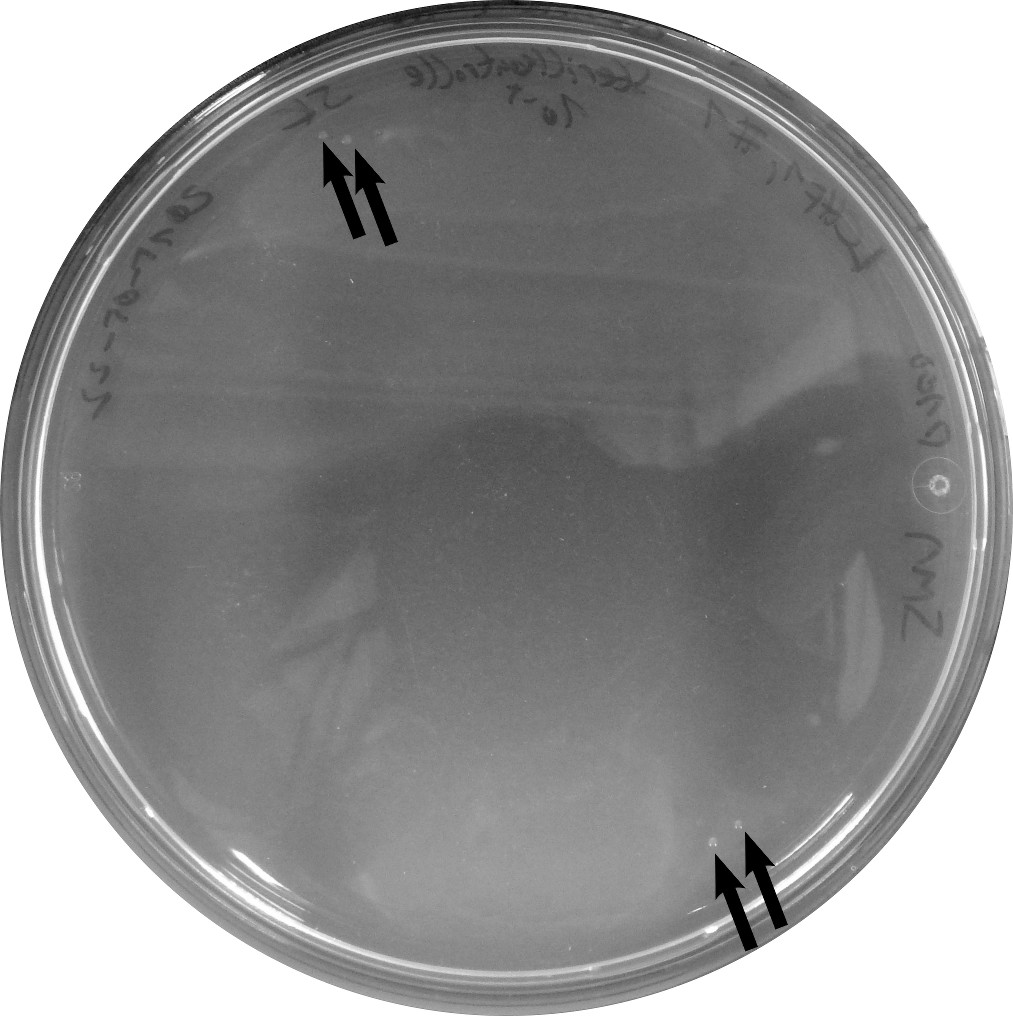
\includegraphics[width=7.0cm]{{fig/7l_15.5h_sterile_control_grey}.jpg}
	}
	\hfill
	\subfloat[\SIh{39.5}. All colonies are exclusively from \strain{}.]{
			\label{fig-lch-eps-disc-7l-sample-3}%
			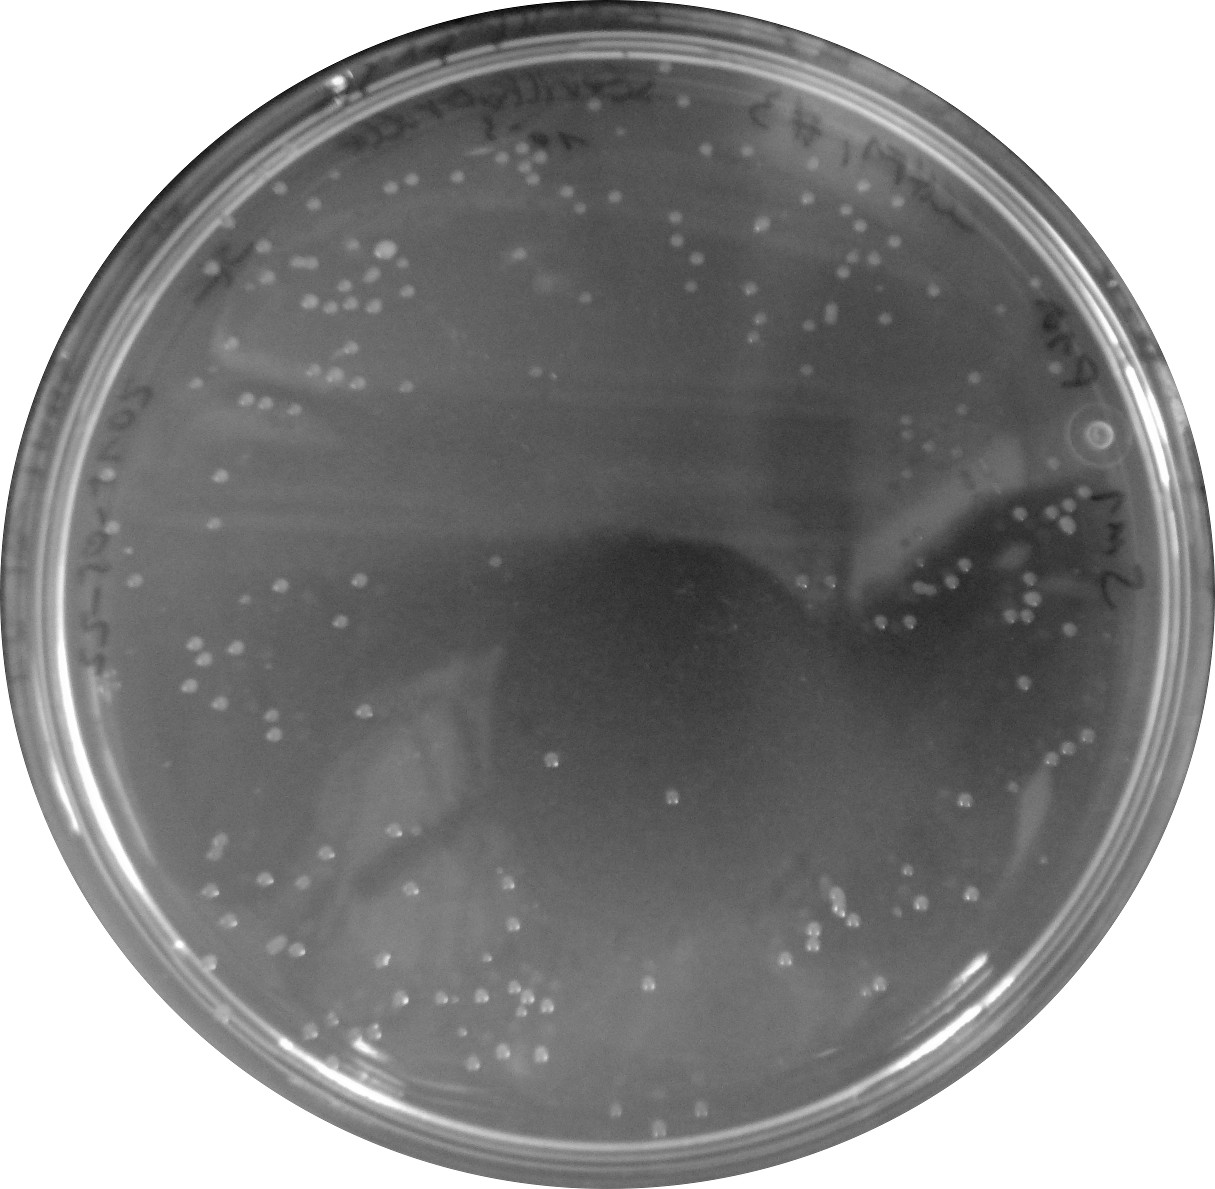
\includegraphics[width=7.0cm]{{fig/7l_39.5h_sterile_control_grey}.jpg}
	}
	\hspace{0.8cm}
	\subfloat[\SIh{53.8}. Arrow: mixed colony of the contaminant and \strain{}. The big and more opaque round colonies surrounding the contaminant colony are from \strain{} exhibiting a different morphology when near the contaminant.]{
			\label{fig-lch-eps-disc-7l-sample-5}%
			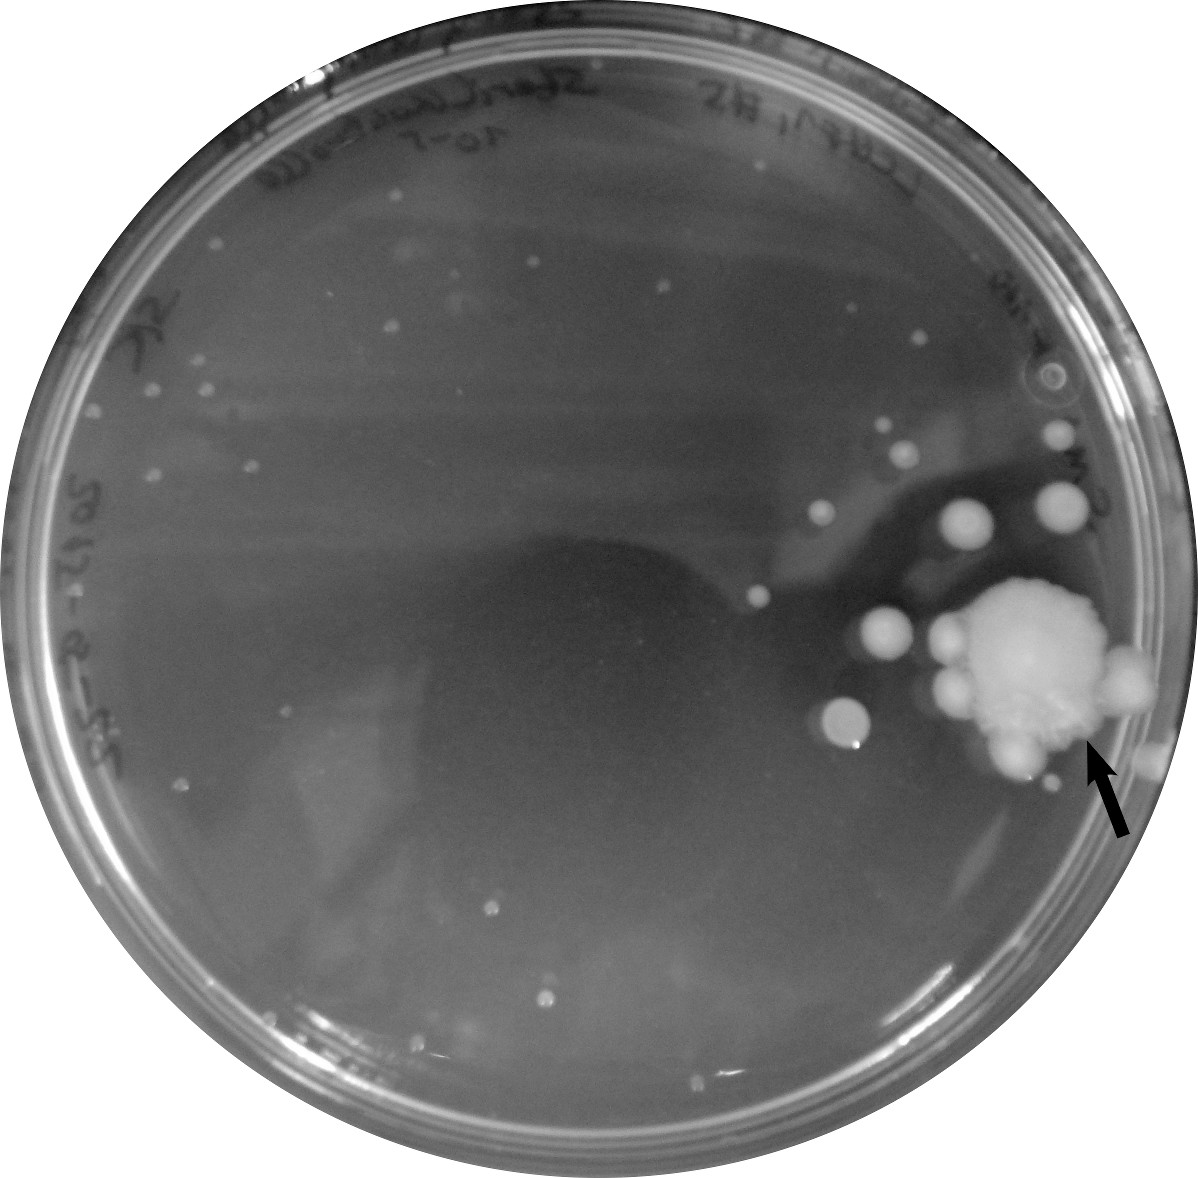
\includegraphics[width=7.0cm]{{fig/7l_53.8h_sterile_control_grey}.jpg}
	}
	\hfill
	\subfloat[\SIh{80.0}. The rosette-like colonies are pure contaminant colonies. The arrows point to mixed colonies of contaminant and \strain{}. Other colonies are from \strain{} mostly exhibiting the same morphology as seen in the \SIh{53.8} sample.]{
			\label{fig-lch-eps-disc-7l-sample-7}%
			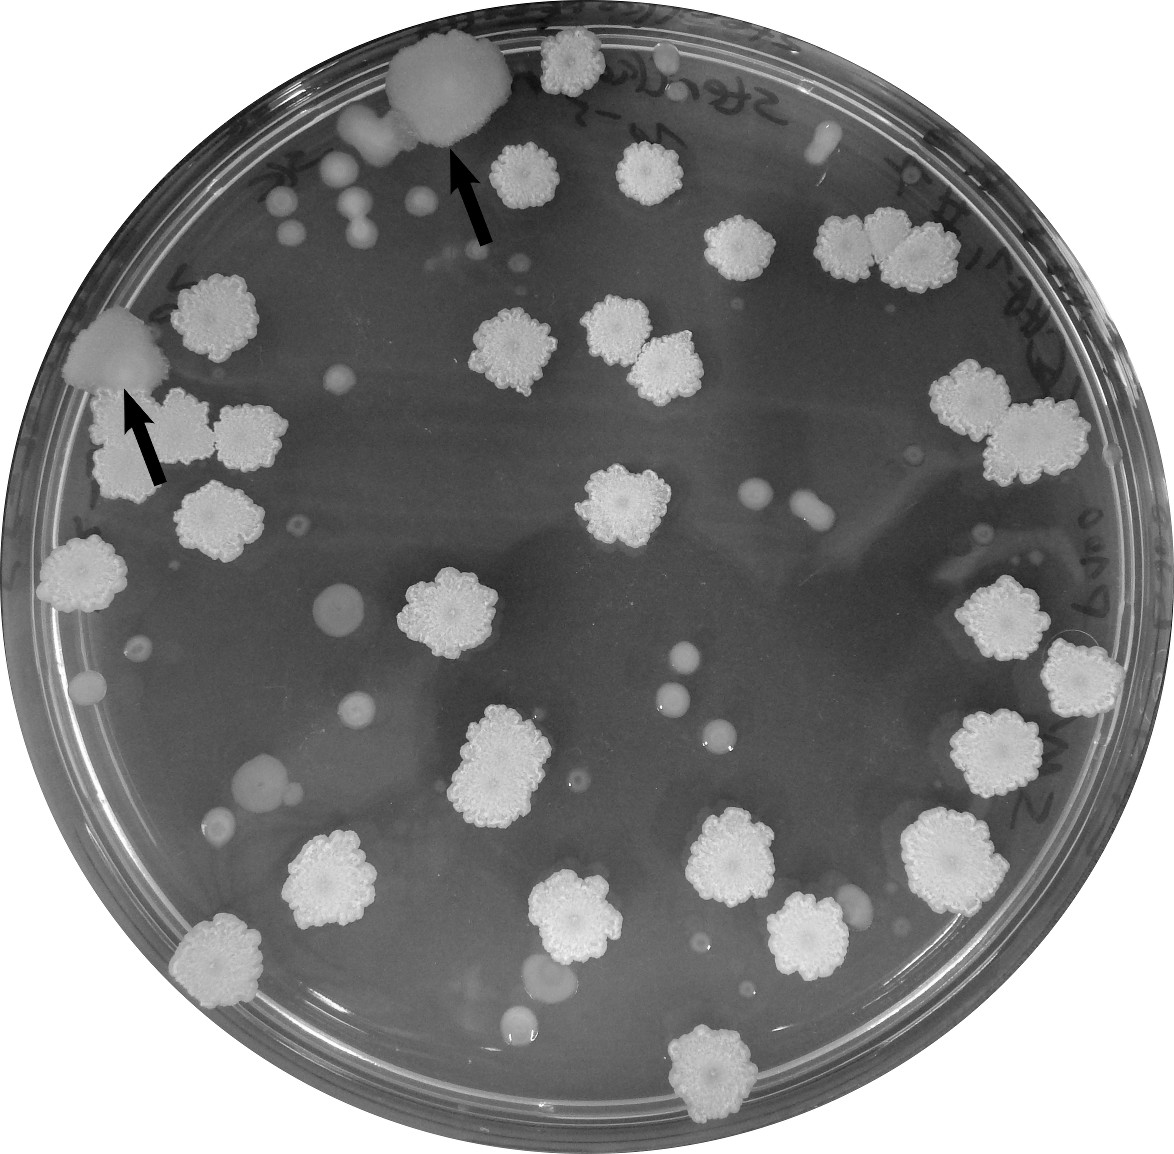
\includegraphics[width=7.0cm]{{fig/7l_80.0h_sterile_control_grey}.jpg}
	}
	\caption[Sterile Controls of the \SIl{7} Fermentation]{
	Sterile controls of the \SIl{7} fermentation.
	\strain{} was fermented at \SIl{7} scale using a fed-batch process.
	The initial volume was \SIl{5.0} with \SIpct{5} \lch{}.
	Starting \SIh{4} after inoculation, \lch{} and medium concentrate were fed linearly increasing for \SIh{24} to a final \lch{} concentration of \SIpct{30}.
	After \SIh{80.0} the fermentation was stopped and the fermentation broth harvested.
	Sterile controls were prepared from \SIul{100} of 1:\num[scientific-notation = true, retain-unity-mantissa = false]{1E5} diluted sample on SM1 P100 agar plates.
	The plates were incubated for \SId{3} at \SIdC{30}.
	\label{fig-lch-eps-disc-7l-contamination}}
\end{figure}

The experiences from the parallel fermentation were used to shorten the lag phase: the fermenter was inoculated with a $D_{600}$ of \num{0.2} instead of \num{0.05} and at the start of the fermentation, only \SIpct{5} \lch{} was supplied. After four hours of incubation and adaptation, the fermenter was fed \lch{} and the corresponding other medium components over the course of the next \SIh{24}, increasing linearly. The final medium contained \SIpct{30} and the strain grew from the beginning.

The reason, why the \SIl{7} fermentation is not part of the results section, is a contamination with a \mo{Bacillus subtilis}. The contamination became visible on a sterile control of the \SIh{53.8} sample. In \vref{fig-lch-eps-disc-7l-contamination}, four SM1 P100 plates at different timepoints of the fermentation are shown. At the end of the fermentation, the contaminant and \strain{} were present in approximately the same number. The 16S rDNA sequence of the contamination is given in \vref{fig-lch-pf-discussion-7l-contamination-16s}. The two best hits in a BLAST search using MegaBLAST in the database \enquote{nt} of NCBI were \mo{Bacillus subtilis} subsp. \mo{inaquosorum} strain 19A\_1.1 and \mo{Bacillus subtilis}~BSn5. Samples up to and including the \SIh{48.0} sample are considered virtually unaffected by the contaminant.

The most likely infection route was the sampling valve at the bottom of the fermenter. A simple test was devised to confirm this assumption. % SK5, S. 155
After the fermentation, sterilization and cleaning, the outlet of the sampling valve was blocked and filled with sterile SM1 P100. After incubation of approximately \SImin{40}, the medium was gathered in a \SIml{50} tube and put on a rocking platform at room temperature for approximately \SIh{7} at \SIrpm{120}. The $D_{600}$ after incubation was \num{0.24}. \SIul{100} was streaked in dilutions of \numrange[scientific-notation = true, retain-unity-mantissa = false, retain-zero-exponent = true]{1E0}{1E-7}. Around \SI[retain-unity-mantissa = false]{1E5}{\CFU\per\milli\litre} and at least four different colony morphologies were found.

While the fermenter was sterilized in place, the tubing could not be sterilized and given prior fermentations in this fermenter with spore-forming bacteria, the issue was aggravated by the high viscosity of the broth. While the tube would drain at the beginning of the fermentation, the viscous broth stayed in the tubing allowing the growth of the contaminating species. Upon the next sampling, the valve was opened and closed again allowing the entry of the contaminant.

Nonetheless, the contamination allowed one interesting observation: the growth of \strain{} was influenced by the contamination and the difference is apparent on the sterile controls as well: colonies grew to larger sizes and had a different colour. While they were translucent white before, when growing in vicinity to the contaminant colony, they would turn to a more yellowish to beige phenotype. Also, the rheological behaviour of the fermentation broth at the end of the fermentation did not resemble anything the author has seen before in a biologically produced polymer solution. Therefore, deliberate co-cultivations might pose yet another method for process optimization \cite{Bader2010}.

In order to verify the assumption that the actual cell dry mass does not decrease, but the slime phase does, the two phases were separated after centrifugation and weighed alone. Although the fermentation was contaminated, weighing both separately allowed to gather some valuable information:
\begin{itemize}
	\item The bottom phase dry mass remained low throughout the fermentation. The low masses made accurate determinations difficult, but until the contamination, the bottom phase dry mass did not exceed \SIgpl{1.0}.
	\item After the contamination, bottom phase dry mass increased until \SIgpl{1.8} at the end of fermentation.
	\item The top phase dry mass exceeded the bottom phase dry mass from the second sample on: until the contamination, the top phase amassed \SIgpl{20.8} dry matter.
	\item With the contamination taking over, the top phase dry mass fell down to \SIgpl{10.2} at the end of the fermentation. The highest value was \SIgpl{35.4}, when the contamination was first visible on plate.
\end{itemize}
The rise of the bottom phase dry mass and the fall of the top phase dry mass coincide suggesting that \strain{} ceased \eps{} production, so that more cells could settle in the bottom phase.

%lch-pf: AUSLASSEN: EPS2.H7 in Datenbank als "Xanthomonas" annotiert, auch Grund für pH-Absenkung; wahrscheinlich nicht haltbar, da kein Paper dazu auftreibbar; einziges Paper dazu geht in die entgegengesetzte Richtung (s. lch-pf)

